\documentclass{beamer}
\mode<presentation>
\usepackage{amsmath,amssymb,mathtools}
\usepackage{textcomp}
\usepackage{gensymb}
\usepackage{adjustbox}
\usepackage{subcaption}
\usepackage{enumitem}
\usepackage{multicol}
\usepackage{listings}
\usepackage{url}
\usepackage{graphicx} % <-- needed for images
\def\UrlBreaks{\do\/\do-}

\usetheme{Boadilla}
\usecolortheme{lily}
\setbeamertemplate{footline}{
  \leavevmode%
  \hbox{%
  \begin{beamercolorbox}[wd=\paperwidth,ht=2ex,dp=1ex,right]{author in head/foot}%
    \insertframenumber{} / \inserttotalframenumber\hspace*{2ex}
  \end{beamercolorbox}}%
  \vskip0pt%
}
\setbeamertemplate{navigation symbols}{}

\lstset{
  frame=single,
  breaklines=true,
  columns=fullflexible,
  basicstyle=\ttfamily\tiny   % tiny font so code fits
}

\numberwithin{equation}{section}

% ---- your macros ----
\providecommand{\nCr}[2]{\,^{#1}C_{#2}}
\providecommand{\nPr}[2]{\,^{#1}P_{#2}}
\providecommand{\mbf}{\mathbf}
\providecommand{\pr}[1]{\ensuremath{\Pr\left(#1\right)}}
\providecommand{\qfunc}[1]{\ensuremath{Q\left(#1\right)}}
\providecommand{\sbrak}[1]{\ensuremath{{}\left[#1\right]}}
\providecommand{\lsbrak}[1]{\ensuremath{{}\left[#1\right.}}
\providecommand{\rsbrak}[1]{\ensuremath{\left.#1\right]}}
\providecommand{\brak}[1]{\ensuremath{\left(#1\right)}}
\providecommand{\lbrak}[1]{\ensuremath{\left(#1\right.}}
\providecommand{\rbrak}[1]{\ensuremath{\left.#1\right)}}
\providecommand{\cbrak}[1]{\ensuremath{\left\{#1\right\}}}
\providecommand{\lcbrak}[1]{\ensuremath{\left\{#1\right.}}
\providecommand{\rcbrak}[1]{\ensuremath{\left.#1\right\}}}
\theoremstyle{remark}
\newtheorem{rem}{Remark}
\newcommand{\sgn}{\mathop{\mathrm{sgn}}}
\providecommand{\abs}[1]{\left\vert#1\right\vert}
\providecommand{\res}[1]{\Res\displaylimits_{#1}}
\providecommand{\norm}[1]{\lVert#1\rVert}
\providecommand{\mtx}[1]{\mathbf{#1}}
\providecommand{\mean}[1]{E\left[ #1 \right]}
\providecommand{\fourier}{\overset{\mathcal{F}}{ \rightleftharpoons}}
\providecommand{\system}{\overset{\mathcal{H}}{ \longleftrightarrow}}
\providecommand{\dec}[2]{\ensuremath{\overset{#1}{\underset{#2}{\gtrless}}}}
\newcommand{\myvec}[1]{\ensuremath{\begin{pmatrix}#1\end{pmatrix}}}
\let\vec\mathbf

\title{MatGeo Presentation - Problem 4.3.55}
\author{EE25BTECH11064 - Yojit Manral}
\date{}

\begin{document}

\frame{\titlepage}
\begin{frame}{Question}
Find the vector equation of the plane passing through the points $\vec{R}\brak{2, 5, -3}$, $\vec{S}\brak{-2, -3, 5}$ and $\vec{T}\brak{5, 3, -3}$.
\end{frame}

\begin{frame}{Solution}
\begin{table}[h!]    
  \centering
  \begin{tabular}[12pt]{ |c| c|}
    \hline
    \textbf{Points} & \textbf{Name}\\ 
    \hline
	\myvec{7\\10} & Point $\Vec{A}$ \\
    \hline 
	\myvec{-2\\5} & Point $\Vec{B}$\\
    \hline
	\myvec{3\\4} & Point $\Vec{C}$\\
    \hline
\end{tabular}
  \caption{List of Points}
  \label{Table_1}
\end{table}\\

$\rightarrow$ We can write the equation for the required plane as
\begin{align} \vec{n}^{T}\vec{x} = c \end{align}
$\rightarrow$ Also, $\vec{R}$, $\vec{S}$ and $\vec{T}$ satisfy this equation. Hence
\end{frame}

\begin{frame}{Solution}
\begin{align}
    \vec{n}^{T}\vec{R} = c \\
    \vec{n}^{T}\vec{S} = c \\
    \vec{n}^{T}\vec{T} = c
\end{align}
$\rightarrow$ From (1), (2), (3) and (4), we get
\begin{align} \vec{n}^{T}\myvec{\vec{R} & \vec{S} & \vec{T}} &= c\myvec{1 & 1 & 1} \end{align}
$\rightarrow$ Using transpose on both sides, we get
\begin{align}
    \myvec{\vec{R} & \vec{S} & \vec{T}}^{T} \vec{n} &= c\myvec{1\\1\\1} \\
    \vec{n} &= c \brak{\myvec{\vec{R} & \vec{S} & \vec{T}}^{T}}^{-1} \myvec{1\\1\\1} 
\end{align}
\end{frame}

\begin{frame}{Solution}
\begin{align}
    &= c \brak{\myvec{2 & -2 & 5 \\ 5 & -3 & 3 \\ -3 & 5 & -3}^{T}}^{-1} \myvec{1\\1\\1} \\
    &= c \myvec{2 & 5 & -3 \\ -2 & -3 & 5 \\ 5 & 3 & -3}^{-1} \myvec{1\\1\\1} \\
    &= \frac{c}{56} \myvec{-6 & 6 & 16 \\ 19 & 9 & -4 \\ 9 & 19 & 4} \myvec{1\\1\\1} \\
    &= \frac{c}{7} \myvec{2\\3\\4}
\end{align}
\end{frame}

\begin{frame}{Solution}
$\rightarrow$ From (11), we get the value of
\begin{align} \vec{n} = \myvec{2 \\ 3 \\ 4} \end{align}
$\rightarrow$ From (2) and (12), we get
\begin{align} c = \myvec{2 & 3 & 4} \myvec{2 \\ 5 \\ -3} = 7 \end{align}
\end{frame}

\begin{frame}{Solution}
\begin{figure}[h!]
   \centering
   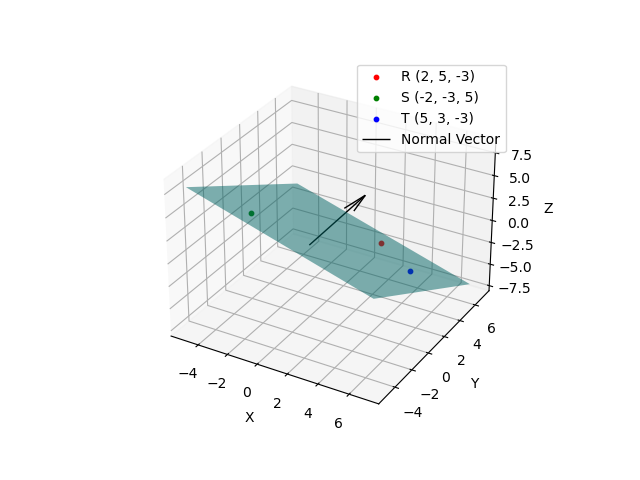
\includegraphics[width=0.7\linewidth]{figs/01.png}
   \caption{Plot of plane $\vec{n}^{T}\vec{x} = c$}
   \label{Plot_1}
\end{figure}
\end{frame}
 % --------- CODE APPENDIX ---------
\section*{Appendix: Code}

% C program
\begin{frame}[fragile]{File: points.c}
\begin{lstlisting}[language=C]
#include <stdio.h>

int main() {
  FILE *fp;

  // -------------------
  // Question 4.3.55
  // -------------------


  fp = fopen("points.dat", "w");
  fprintf(fp, "%d,%d,%d\n", 2, 5, -3);  // R
  fprintf(fp, "%d,%d,%d\n", -2, -3, 5);   // S
  fprintf(fp, "%d,%d,%d\n", 5, 3, -3); // T
  fclose(fp);
  return 0;
}
\end{lstlisting}
\end{frame}

% Python calling C
\begin{frame}[fragile]{File: call\_c.py}
\begin{lstlisting}[language=Python]
import subprocess

# Compile the C program
subprocess.run(["gcc", "points.c", "-o", "points"])

# Run the compiled C program
result = subprocess.run(["./points"], capture_output=True, text=True)

# Print the output from the C program
print(result.stdout)
\end{lstlisting}
\end{frame}

% Python plotting
\begin{frame}[fragile]{File: plot.py}
\begin{lstlisting}[language=Python]
import numpy as np
import matplotlib.pyplot as plt
from mpl_toolkits.mplot3d import Axes3D

# Define the points
R = np.array([2, 5, -3])
S = np.array([-2, -3, 5])
T = np.array([5, 3, -3])
normal = np.array([2, 3, 4])
# Create a grid to plot the plane
x = np.linspace(-5, 7, 10)
y = np.linspace(-5, 7, 10)
X, Y = np.meshgrid(x, y)

# Equation of the plane: Ax + By + Cz = D
A, B, C = normal
D = np.dot(normal, R)

# Solve for Z
Z = (D - A * X - B * Y) / C

# Plotting the plane and the points R, S, T
fig = plt.figure()
ax = fig.add_subplot(111, projection='3d')

# Plot the points
ax.scatter(*R, color='r', label='R (2, 5, -3)', s=10)
ax.scatter(*S, color='g', label='S (-2, -3, 5)', s=10)
ax.scatter(*T, color='b', label='T (5, 3, -3)', s=10)
\end{lstlisting}
\end{frame}

% Python plotting
\begin{frame}[fragile]{File: plot.py}
\begin{lstlisting}[language=Python]
# Plot the plane
ax.plot_surface(X, Y, Z, alpha=0.5, rstride=100, cstride=100, color='c')

# Plot the normal vector starting from point R
ax.quiver(0, 0, 0, normal[0], normal[1], normal[2], color='k', length=1, linewidth=1, label='Normal Vector')

# Labels and legend
ax.set_xlabel('X')
ax.set_ylabel('Y')
ax.set_zlabel('Z')
ax.legend()

# Display plot
plt.show()
\end{lstlisting}
\end{frame}
\end{document}
